\documentclass[11pt, oneside]{article} 
\usepackage{geometry}
\geometry{letterpaper} 
\usepackage{graphicx}
	
\usepackage{amssymb}
\usepackage{amsmath}
\usepackage{parskip}
\usepackage{color}
\usepackage{hyperref}

\graphicspath{{/Users/telliott/Github/precalculus/fig/}}

\title{Equal sides}
\date{}

\begin{document}
\maketitle
\Large

There are several adjectives one can use to describe different types of triangles.  For example:  acute, right, and obtuse.  
\begin{center} 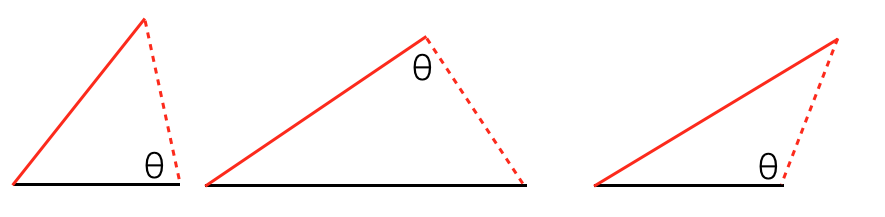
\includegraphics [scale=0.4] {tri_types.png} \end{center}

The acute triangle (left) has all three angles smaller than a right angle.  The right triangle, naturally, has one right angle (it can't have two --- why?)

We'll say a lot more about right triangles later.

Finally, an obtuse triangle has one angles larger than a right angle (right, above).

\subsection*{symmetry}

One can also talk about the situation where either two sides, or all three sides, have the same length.  

An equilateral triangle has all three sides the same, while an isosceles triangle has two sides the same length.

The most important consequence of three sides equal for an equilateral triangle, is rotational symmetry.  Three turns of $120$ degrees, and we're back where we started.

\begin{center} 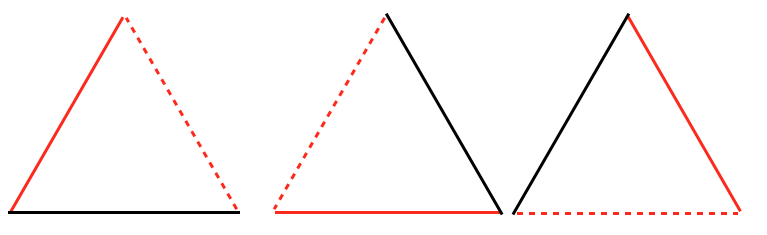
\includegraphics [scale=0.4] {equilateral.png} \end{center}

The implication of that is that the three angles are also equal.  There is no reason to choose one larger than the other.

In the next figure the two smaller triangles obtained by dividing in half an equilateral triangle (all sides equal), are congruent.

\begin{center} 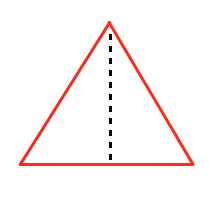
\includegraphics [scale=0.6] {congruent2.png} \end{center}

By divide in half, we mean bisect the base and draw the line from the top vertex.  We have SSS.

\subsection*{circumscribed circle}

Here is a fun construction for an equilateral triangle.  Any triangle fits into a unique circle.  We will prove this elsewhere.

\begin{center} 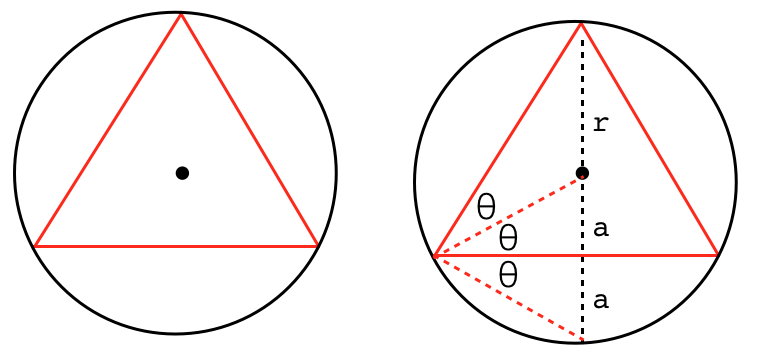
\includegraphics [scale=0.4] {one_third.png} \end{center}

If we draw the radius to a vertex of the triangle, and then to the end of the diameter, it looks tantalizing.

Here is the proof.  

First, the radius is an altitude, and it divides the vertex angle in half, as we've been saying.  So that accounts for two of the angles labeled $\theta$.  The third comes about because any triangle with two points on the diagonal and a third anywhere on the circle is a right triangle.  We'll prove that when we get to circles.

As a result, by measure $\theta$ is $30$ degrees.  Since a right triangle is $90$, we assign the third $\theta$.

\begin{center} 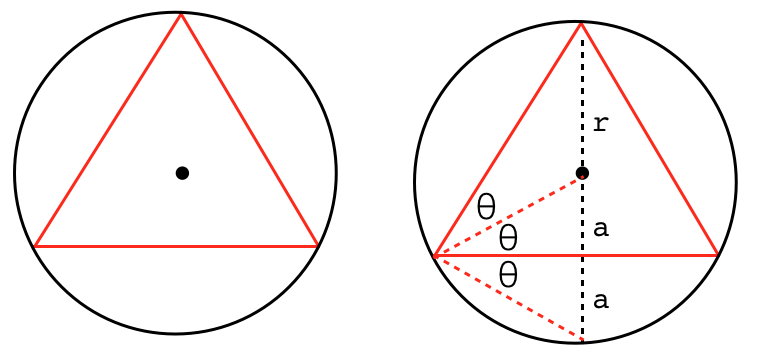
\includegraphics [scale=0.4] {one_third.png} \end{center}

So now we have a smaller angle of a right triangle, and a shared side.  The two triangles are congruent.  That accounts for the duplicated $a$ in the figure.

Thus, the altitude of the equilateral triangle is $3/4$ of the diameter of the circle that just encloses it.  And the point where the altitudes meet in an equilateral triangle is $1/3$ of the way up from the base, since $r = 2a$.  

We will see that such a point where the altitudes cross is unique and exists for any triangle, and it always has the same measure as a fraction of the altitude.  This is called Ceva's theorem.

\subsection*{theorem from Thales}

$\bullet$  The base angles of an isosceles triangle are equal.  Also, if the two base angles are equal, the triangle is isosceles.

\begin{center} 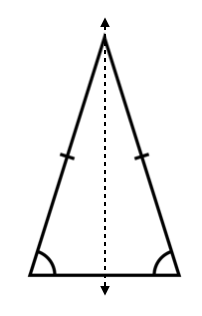
\includegraphics [scale=0.6] {isosceles.png} \end{center}

My favorite proof of this theorem is from reflective or mirror image symmetry (above).  

Start with the two sides equal and draw a line to the midpoint of the base opposite.  The figure has reflective symmetry, thus the angle is bisected.

We prove this more carefully now.

\subsection*{notation}

The Greeks, including Euclid, adhere to certain conventions.  For example, points are always labeled with letters, line segments are referred to by the endpoints, and angles by the line segments that determine them, as in $\angle ABC = \angle DEF$.

I don't know about you but I find myself tracing out angles from the three points, again and again.

We could give labels to the angles like $\alpha, \beta \dots$, and to the sides opposite vertices as $a$ opposite $A$ and so on.  

But let's go with something even more dramatic.  Dispense with labels altogether and use colored dots for equal angles and colored bars for equal lengths.  We give the famous proof of Thales' theorem from Euclid's \emph{Elements}.

\subsection*{Prop. I.5}

In isosceles triangles the angles at the base equal one another, and, if the equal straight lines are produced further, then the angles under the base equal one another.

In what follows, all the pieces are with reference to the initial construction, first figure, below.

\begin{center} 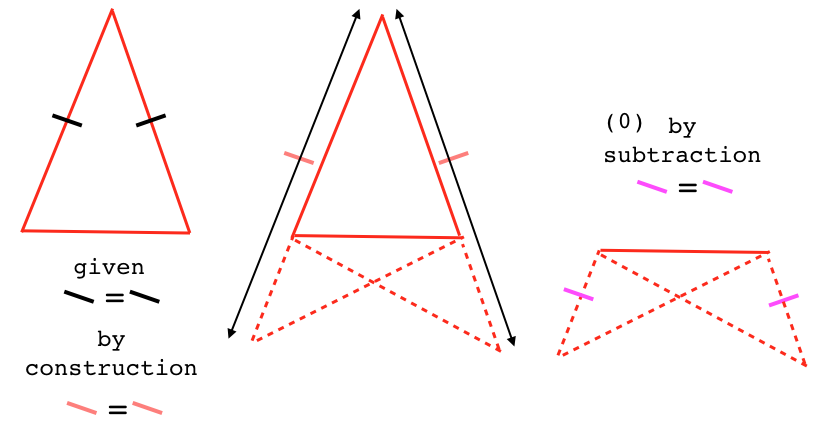
\includegraphics [scale=0.35] {PI_5d.png} \end{center}

\begin{center} 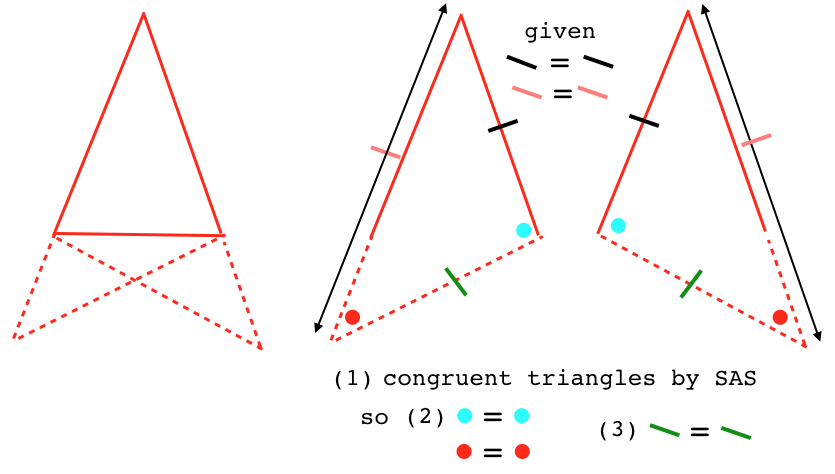
\includegraphics [scale=0.35] {PI_5e.png} \end{center}

\begin{center} 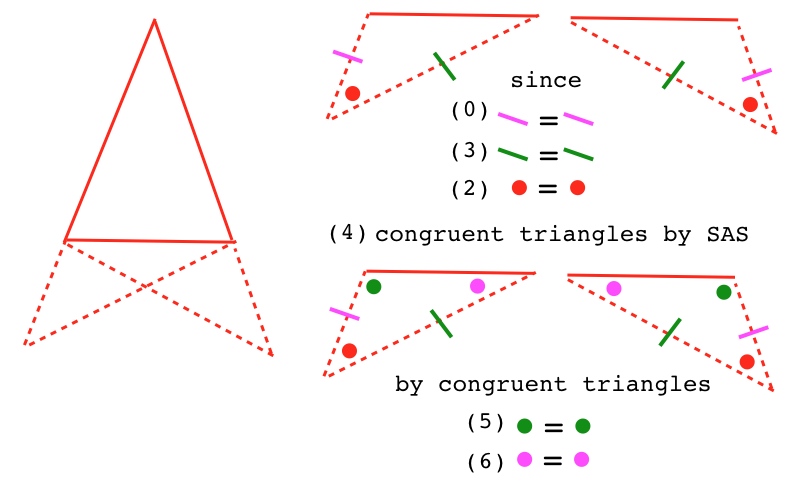
\includegraphics [scale=0.35] {PI_5f.png} \end{center}

\begin{center} 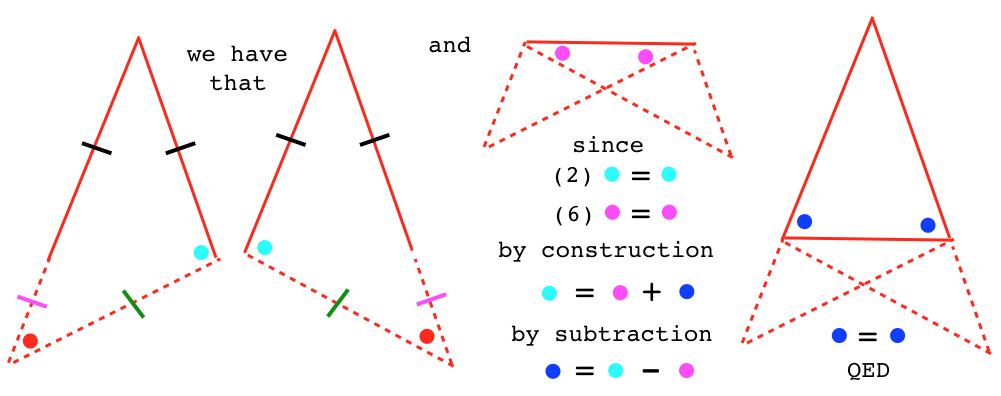
\includegraphics [scale=0.35] {PI_5g.png} \end{center}

$\square$

The theorem says that the base angles are equal $\iff$ the two sides sides are equal (not the base).  

The symbol $\iff$ means \emph{if and only if}, so $A \iff B$ means that both $A \rightarrow B$ and $B \rightarrow A$.

Above we said that in this figure the two smaller triangles obtained by dividing an equilateral triangle in half, are congruent.  The dotted line is called an \emph{altitude} of the triangle.

\begin{center} 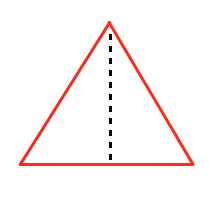
\includegraphics [scale=0.5] {congruent2.png} \end{center}

An altitude meets the side opposite in a right triangle.

Because the left and right sides of the original triangle are equal, the base angles are equal, by the property of isosceles triangles which we just proved.  The angles where the altitude meets the base are both right angles, by symmetry and by the definition of the altitude.  

Therefore we have AAS, and the two halves are congruent.

So, the two angles at the top where the altitude meets the sides are also equal (as the third angle with the other two angles determined).


\end{document}